\documentclass[tikz]{standalone}
\usepackage{pgfplots}
\pgfplotsset{compat=1.15}
\usepackage{mathrsfs}
\usetikzlibrary{arrows,calc}
\usepackage{tkz-euclide}

\pagestyle{empty}

\definecolor{AngleClr}{rgb}{0,0.39215686274509803,0}
\definecolor{ShapeClr}{rgb}{0.6,0.2,0}

\begin{document}

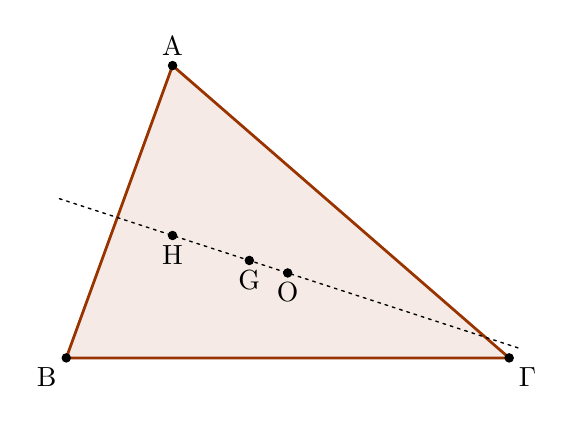
\begin{tikzpicture}[scale=.75]
\tkzSetUpLine[line width=1pt,color=black]
\tkzSetUpPoint[fill=black]

\tkzDefPoints{0/0/B,1.8/4.95/A,7.5/0/C}

\tkzDefTriangleCenter[circum](A,B,C) \tkzGetPoint{O}
\tkzDefTriangleCenter[centroid](A,B,C) \tkzGetPoint{G}
\tkzDefTriangleCenter[ortho](A,B,C) \tkzGetPoint{H}


\tkzDefMidPoint(B,C) \tkzGetPoint{MA}
\tkzFillPolygon[fill=ShapeClr,fill opacity=0.1](A,B,C)

\tkzDrawPolygon[color=ShapeClr](A,B,C)

\tkzDrawSegments[line width=0.5pt,color=black,dashed,dash pattern=on 1pt off 1.75pt,add=2 and 1](O,H)

\tkzDrawPoints[size=3](A,B,C,H,G,O)
\tkzLabelPoint[above](A){$\rm A$}
\tkzLabelPoint[below left](B){$\rm B$}
\tkzLabelPoint[below right](C){$\rm \Gamma$}
\tkzLabelPoint[below](O){$\rm O$}
\tkzLabelPoint[below](H){$\rm H$}
\tkzLabelPoint[below](G){$\rm G$}


\end{tikzpicture}

\end{document}
